% Appendix D

\chapter{Analysing double-strand breaks in cultured cells for drug screening applications by causual inference} % Main appendix title
\chaptermark{Analysing double-strand breaks}
\label{AppendixD} % For referencing this appendix elsewhere, use \ref{AppendixA}

%\lhead{Appendix C. \emph{Statistical Tests}} % This is for the header on each page - perhaps a shortened title

\emph{The contents of this appendix were published in the Proceedings of the 14th IEEE International Symposium on Biomedical Imaging (ISBI). Washington D.C., United State of America. April, 2018. \\ \\ Double strand breaks (DSB) are a hallmark of DNA damage and genetic instability, which are important features of cancer cells.  In addition, repair of DSBs provide interesting therapeutic targets. Fluorescence microscopy allows us to visualise DSBs in cells using a dedicated fluorescent marker, which is therefore an informative readout for drug screening applications. We therefore need robust methods in image analysis and statistical analysis to quantify DSBs in single cells and thereby to assess the drug effect with respect to the related pathways. The contribution of this paper is two-fold: first, we compare different DSB quantification schemes; and second we provide a sound statistical framework based on causal inference in order to detect drugs acting directly on DSBs. In particular this second aspect is so far notoriously neglected in the field, even though it is essential for the specific assignment of the drug effect.}

\section{Introduction}
%\subsection{Introduction}
%\label{subsec:intro}

 Dysfunction of the DNA repair mechanisms is a major hallmark of cancer. Monitoring DNA damage by fluorescently labeling double strand breaks (DSB) in cells is therefore an important readout in drug screening of cancer cell lines. DSBs  occur when both strands of the DNA double helix are broken. DSBs have various causes, for example, cytotoxic radiation, or DNA replication over an existing single-strand break. Despite the natural DNA repair mechanisms of the cell, DSBs can be irreparable, leading ultimately to apoptosis, or hazardous DNA rearrangements. As such, DSBs are an interesting property to assess when analysing the effects of small compounds upon cancer cells.

The context of this research is a drug screen in triple-negative breast cancer (TNBC), a type of cancer that is characterised by the absence of genetic markers that are common targets for cancer therapies. The difficulty of treatment of TNBC make the search for effective new treatments particularly important. It must be noted however that DSB quantification is not limited to this application; it is a general marker often used in cancer research, and in particular in screening applications. 


%In a drug screen, one indicator of drug cytotoxicity is an increase of DNA damage in the form of double-strand breaks (DSB). Such damage occur when both strands of the DNA double helix are broken. DSBs have various causes, for example, cytotoxic radiation, or DNA replication over an existing single-strand break. Despite the natural DNA repair mechanisms of the cell, DSBs can be irreparable, leading ultimately to apoptosis, or a hazardous mutation. As such, DSBs are an interesting property to assess when analysing the effects of small compounds upon cancer cells.

In Section \ref{sec:experimental} we describe the experimental setup of the drug screen. In Section \ref{sec:approaches} we compare three approaches to quantifying DSBs over the imaged cell populations.
%: counting high-intensity spots, granulometric features, and a straightforward normalised average intensity. 
% this cannot be understood at this moment in the paper:
%These are computed on the cyanine 3 channel of our image dataset. 
%In drug screen applications, many severely perturbed cells - such as mitotic or dead cells - are typically washed away prior to image acquisition.
%A washing step of the experimental protocol generally precludes detection of apoptotic cells, as these become unfastened and washed away. 
Then, we show that analysis of DSB numbers can be misleading for two reasons: first, the number of DSBs may depend on the cell cycle and drugs assigned to affect DSBs might actually only affect the cell cycle. Second, in drug screening, severely perturbed cells--such as mitotic or dead cells--are typically washed away prior to image acquisition. Such a \emph{loss to followup} introduces a potential selection bias when performing significance tests. Both aspects have been neglected so far in the drug screening literature (\cite{avondoglio2009high}, \cite{garcia2013assessment}). We use the tools of causal inference to probe for such systematic bias in our analysis in Section \ref{sec:analysis}. A comparison of the DSB quantifiers used and the analytic corrections are presented in Section \ref{sec:results}. Closing remarks are given in Section \ref{sec:conclusions}.

\section{Experimental setup}
\label{sec:experimental}

In a pilot study on multiple TNBC cell lines, we assembled 168 drugs, including two positive controls, for a drug screen at high concentration ($10\mu M$), alongside replicated negative controls of neutral agent \emph{dimethyl sulfoxide} (DMSO) and untreated cells. The wells were seeded with a controlled 1000 and 1250 cells for MDA231 and MDA468 cell lines respectively, on separate 384-well microplates. The drugs were administered identically on both plates. Following hibernation, the cells were fixed, washed, and stained with four fluorescent markers. Fluorescence microscopy ($20\times$ widefield with deconvolution image restoration) taken at four fields in each well produced two experimental datasets of 1536 multiplexed images apiece.

Four fluorescent stains were used for our microscopy: DAPI, Cyanine 3 (Cy3), Cyanine 5 (Cy5), and FITC. Of interest to our analysis are DAPI and Cy3, fluorescent markers for DNA and DSBs, respectively.

The final, washing step evacuates all unfastened cells from the well, such as mitotic or dead cells, as a consequence of perturbation or otherwise. The array of perturbations show a range of effects on cell mortality, from no apparent effect to a near or complete elimination of cells.

\section{Approaches to measuring double-strand breaks}
\label{sec:approaches}

While biochemical techniques exist for DSB quantification (\cite{chailleux2014quantifying}), obtaining faithful counts of DSBs directly from bioimages is problematic as the correspondence between DSBs and the recorded signal is unclear. Our strategy is therefore to extract a feature that has a high chance of being proportional to the amount of DSBs. The Cy3 signal typically manifests as a nebulous cloud, with intermittent peaks or spots of higher intensity. Samples are given in Figure \ref{fig:spots}. DSBs may be underrepresented by a simple spot count, as high intensity spots may correspond with multiple, localised breaks. On the other hand, DSBs may be overrepresented by a noisy Cy3 channel. We here compare three approaches to quantifying double-strand breaks. The approaches give correlated readouts, in particular between spot count and granulometry (Figure \ref{fig:corr}) with $\rho=0.84$ over the entire plate, and it seems that any will serve as a reasonable proxy to the true number of DSBs. Granulometry and spot density correlate with average intensity at $\rho=0.44$ and $\rho=0.42$ respectively. 

In general, the features differ most in the rare cases when the marker is saturated and nothing stands out to be counted as a spot, yet the average intensity is artificially high (staining artifacts). We therefore give preference to spot-related features. The computation was performed by Cell Cognition (\cite{held2010cellcognition}), an open-source tool for the visualisation and analysis of HCS assays. As part of a standard computational pipeline, individual cell nuclei were first segmented by a combination of filtering and local thresholding (\cite{held2010cellcognition}). Touching nuclei are split as described in \cite{Naylor2017}, using morphological local contrast dynamics (morphological dynamics) giving superior results to the traditional approach of filtering the Euclidean distance map (data not shown). DSB analysis was then performed for each individual nucleus.

\begin{figure}[b!]
\centering
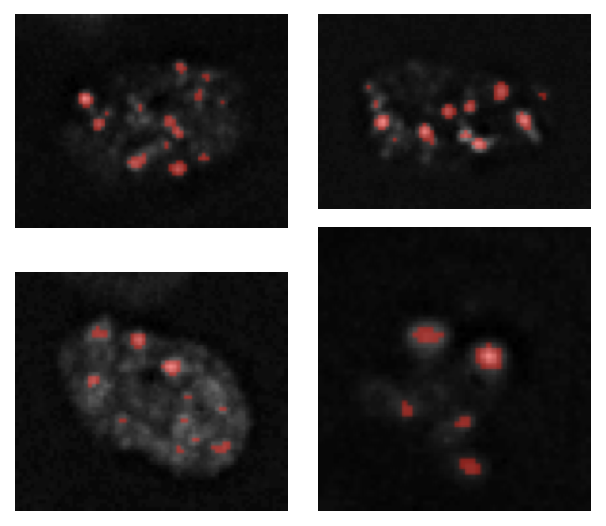
\includegraphics[width=0.8\textwidth]{img/spots.png}
\caption{Examples of spots (red) on cell nuclei detected with diameter openings on the Cy3 channel (grey).}
\label{fig:spots}
\end{figure}

%\begin{figure}[ht]
%\centering
%\includegraphics[width=\linewidth]{img/correlation.pdf}
%\caption{Examples of spots (red) on cell nuclei detected with diameter openings on the Cy3 channel (grey).}
%\label{fig:corr}
%\end{figure}
%\vspace{-.5cm}

\begin{figure}[ht]
\centering
\begin{tikzpicture}
    \begin{axis}[
            axis x line=middle,
            axis y line=middle,
            enlarge y limits=true,
            width=\linewidth, height=8cm,     % size of the image
            grid=major,
            grid style={dashed, gray!30},
            ylabel=granulometry (3),
            xlabel=spot density
         ]        
        \addplot[only marks, mark size=1] table {data/scatter.dat};
        \addplot [no markers, red] table [y={create col/linear regression={y=y}}] {data/scatter.dat};
    \end{axis}
\end{tikzpicture}
\caption{Granulometry and spot density readouts show high correlation on average over all wells.}
\label{fig:corr}
\end{figure}

\subsection{Counting spots with diameter openings}

One approach to measuring DSBs is to count individual spots. For this, we used \emph{diameter openings} (\cite{Walter2007}), a technique based on a similar flooding technique to the watershed algorithm, with the notable difference that no separation of regions is built and that the flooding stops as soon as the maximal extension of the region exceeds a user-defined diameter $\lambda$. Mathematically, the operator can be written as:
\begin{eqnarray} 
  \left[ \gamma^{\circ}_{\lambda}(f) \right] (x) 
    &=& \sup \left\{ s \leq f(x)
        \setsep  \alpha \left( C_x \left[ X_s^+(f) \right] \right) \geq
        \lambda \right\} \nonumber \\ 
    &=& \bigcup \{ \gamma_B(f) \setsep \alpha(B) \geq \lambda \} \label{diameter_open:relation}
\end{eqnarray}
where $X_s^+(f)$ is the set of all pixels with with $f(x)\geq s$, $C_x[A]$ is the connected component of set $A$ containing point $x$ and $\alpha(C_x)$ its maximal extension. Equation \ref{diameter_open:relation} shows that this can also be written as the supremum of \emph{all} morphological openings $\gamma_{B_i}(f)$ with structuring elements $B_i$ whose diameter greater or equal to $\lambda$. 

Building the difference to the original image $f-\gamma^{\circ}_{\lambda}(f)$ and a simple threshold operation thus allows one to extract all bright details with a maximal extension smaller than a certain value. The tunable parameters of the algorithm are the diameter of the structuring element and the value of the intensity threshold\footnote{These were manually tuned to a diameter of 5 pixels, and threshold of 8.}. Nuclei happen to have different sizes and we thus normalise the spot count into \emph{spot density} by dividing by the nuclear area.

\subsection{Granulometry-based features}

An alternative strategy to get a proxy of DSB numbers without relying on hard segmentation, is to use \emph{morphological granulometries}, i.e. the sum of the difference between opened versions of the initial image.
\begin{equation}
\sum_{x \in S_k} \gamma_{B_i}f(x) - \gamma_{B_{i+1}}f(x)
\end{equation}
where the structuring elements $B_i$ fulfill the condition $B_{i} \subset B_{i+1}$ and $S_k$ is the k-th cell.  

\subsection{Average intensity}

We also hypothesised that an accumulation of $\gamma$-H2AX can be seen as an indicator of DNA breaks without a detectable organisation into spots, in particular in the case of very high densities. We therefore added the average intensity over the region of interest as a feature.
\begin{equation}
\frac{1}{\#S_k}\sum_{x \in S_k}f(x)
\end{equation}

\section{Analysis}
\label{sec:analysis}

The aim of our analysis is to compare DSB levels from drug perturbations to levels in the negative control, DMSO. We used the Kolmogorov-Smirnov (K-S) test as the basis of comparison with significance declared at the 0.01 level.

\begin{figure}%
    \centering
    \subfloat[mCherry and GFP fluorescence (left and center) and phase contrast signals (right) at $t = 0$]{
        \begin{tikzpicture}
            \begin{axis}[
                   scale only axis,
                   enlargelimits=false,
                   axis x line=middle,
                   axis y line=middle,
                   width=0.4\linewidth,     % size of the image
                   grid=major,
                   grid style={dashed, gray!30},
                   xlabel=total intensity,
                   xlabel near ticks,
                   font=\footnotesize,
                   restrict y to domain=0:4e-5
                   ]
            \addplot[no markers] table [x, y] {data/hist.dat};
            \addplot[ybar interval, fill=black!10] table [x, y, col sep=comma] {data/hist2.csv};
            \end{axis}
        \end{tikzpicture}
        \label{fig:bimodal}
    }
    \hfill
    \subfloat[mCherry and GFP fluorescence (left and center) and phase contrast signals (right) at $t = 70$]{
        \begin{tikzpicture}
        \begin{axis}[
               scale only axis,
               enlargelimits=false,
               axis x line=middle,
               axis y line=middle,
               width=0.4\linewidth,     % size of the image
               grid=major,
               grid style={dashed, gray!30},
               xlabel=spot density,
               xlabel near ticks,
               font=\footnotesize
            ]        
           \addplot[no markers, mark size=1, black] table {data/kde1.dat};
           \addplot[no markers, mark size=1, red] table {data/kde2.dat};
        \end{axis}
        \end{tikzpicture}
        \label{fig:phases}
    }
  \caption{Distribution of cell total intensities on the DAPI channel for MDA231 cell line (a). The bimodal distribution is a consequence of the growth sustained between the G$_1$ (black) and G$_2$ (red) phases of the cell cycle. A suitable threshold of DAPI intensity significant divergence in the DSB distributions of the respective groups on the Cy3 channel (b).}
\end{figure}

%\begin{figure}[t!]
%\centering
%  \begin{subfigure}[t]{0.45\linewidth}
%    \begin{tikzpicture}
%    \begin{axis}[
%            scale only axis,
%            enlargelimits=false,
%            axis x line=middle,
%            axis y line=middle,
%            width=0.85\linewidth,     % size of the image
%            grid=major,
%            grid style={dashed, gray!30},
%            xlabel=total intensity,
%            xlabel near ticks,
%            font=\footnotesize,
%            restrict y to domain=0:4e-5
%            ]
%    \addplot[no markers] table [x, y] {data/hist.dat};
%\addplot[ybar interval, fill=black!10] table [x, y, col sep=comma] {data/hist2.csv};
%    \end{axis}
%    \end{tikzpicture}
%%    \centering
%%    \includegraphics[width=\linewidth]{img/bimodal.pdf}
%    \caption{}
%    \label{fig:bimodal}
%  \end{subfigure}
%~
%\centering
%  \begin{subfigure}[t]{0.45\linewidth}
%  \begin{tikzpicture}
%    \begin{axis}[
%            scale only axis,
%            enlargelimits=false,
%            axis x line=middle,
%            axis y line=middle,
%            width=0.85\linewidth,     % size of the image
%            grid=major,
%            grid style={dashed, gray!30},
%            xlabel=spot density,
%            xlabel near ticks,
%            font=\footnotesize
%         ]        
%        \addplot[no markers, mark size=1, black] table {data/kde1.dat};
%        \addplot[no markers, mark size=1, red] table {data/kde2.dat};
%    \end{axis}
%  \end{tikzpicture}
%%    \centering
%%    \includegraphics[width=\linewidth]{img/phases.pdf}
%    \caption{}
%    \label{fig:phases}
%  \end{subfigure}
%  %\caption{Distribution of cell total intensities on the DAPI channel for MDA231 cell line (a). The bimodal distribution is a consequence of the growth sustained between the G$_1$ (black) and G$_2$ (red) phases of the cell cycle. A suitable threshold of DAPI intensity significant divergence in the DSB distributions of the respective groups on the Cy3 channel (b).}
%\end{figure}

As can be seen in Figure \ref{fig:bimodal}, there is a bimodal distribution in DAPI intensity considered over all cells, corresponding to cell cycle phases (pre- and post-DNA synthesis). The higher frequency of low intensities corresponds to the longer G$_1$ phase and more cells will be fixed in this phase. Secondly, the DNA content in this phase is constant, whereas the DNA content in S-phase is somewhere between G$_1$ and G$_2$. Third, there are many aberrant morphologies, for which the DNA content is larger than the one of normal G$_1$ cells, but the exact value is not clearly determined. All of these elements lead to a wide distribution of DAPI intensities for all nuclei that are not in G$_1$. We can roughly estimate a suitable threshold between the two classes to create high and low intensity groups. Visualising the respective spot densities for these groups (Figure \ref{fig:phases}) reveals a shift in DSB distribution between the groups.

\subsection{Causal considerations}

Causal inference (\cite{pearl2009causal}) is a framework for conducting statistical analysis that enables reasoning about causal factors in an experimental setting, so as to determine a relationship between a potential cause or \emph{treatment} and a potential effect or \emph{outcome}. Such an analysis is necessarily first endowed with a directed, acyclic causal graph, such as Figure \ref{fig:bias}, by a domain expert. The causal graph postulates a feasible causal relation, respecting the otherwise impossible task of establishing causations from statistical data alone (\cite{pearl2009causal}). In particular, causal models help to identify biases and necessary adjustments in analysis.

One aspect we looked into was the simultaneous effect of perturbations on cell death and DSBs, themselves potentially a cause of cell death. Due to the washing step in the experimental protocol, our observations are confined to those cells surviving the cytotoxic effect, that is, not undergoing apoptosis $A$. This is an example of \emph{selection bias}, whereby the phenomenon of apoptosis determines those cells available for measurement. The bias is illustrated in Figure \ref{fig:bias}, which traces a path from perturbation $P$ to apoptosis $A$, both via DSBs levels $D$, as well as directly, in a path representing other, unmeasured, cytotoxic causes.

\begin{figure}[b!]
\centering
\begin{tikzpicture}[font=\sffamily, square/.style={regular polygon, regular polygon sides=4}]
\node (P) at (0, 0) {P};
\node (D) at (2, 0) {D};
\node (A) [square,draw] at (4, 0) {A};
\draw[-Latex] (P) to (D);
\draw[-Latex] (D) to (A);
\draw[-Latex] (P) to [out=45, in=135] (A);
\end{tikzpicture}
\caption{Causal diagram including selection bias: $P$ is the perturbation; $D$ is the distribution of double-strand breaks and; $A$ is the frequency of apoptosis. Conditioning (represented as a square) on the common effect of treatment $P$ and outcome $D$ creates a selection bias.}
\label{fig:bias}
\end{figure}

In certain scenarios, a selection bias may be corrected for by standardisation or IP-weighting, giving an unbiased estimate of the causal effect. However, the particular causal structure we observe here defies correction, as the levels of $A$ (cell death or not) are not \emph{exchangeable} with respect to $D$, a necessary condition for corrective techniques. This clearly indicates the need for experimental techniques where apoptotic cells remain observable. Despite this bias, independent analyses showed little difference in the distributions of DSBs within sparse (therefore highly apoptotic) and dense cell populations.

Another use case is in the effect of the cell cycle phase: given that some perturbations $P$ affect the cell cycle phase $G$, and that DSBs levels $D$ are influenced by both $P$ and $G$, cell cycle variability acts as an \emph{effect modifier} on $D$. These relations are expressed in the causal graph in Figure \ref{fig:effectmodification}. Though they are not a source of systematic bias, identifying effect modifiers can lead to an insightful stratified analysis. Through stratification, we were able to determine whether increased DSBs levels were a direct effect of perturbation, or an indirect effect of a modified cell cycle. In a stratified analysis, we compared the pooled cells of DMSO wells, as untreated subjects, with the cells of each perturbed well in turn. As we assessed 168 small compound perturbations, a multiple testing correction is due in our analysis. We compensate with the Benjamini-Hochberg correction for controlling the false discovery rate. We compare the effect of stratification in Section \ref{sec:results}.

\begin{figure}
\centering
\begin{tikzpicture}[font=\sffamily, square/.style={regular polygon,regular polygon sides=4}]
\node (P) at (0, 0) {P};
\node (G) at (2, 0) {G};
\node (D) at (4, 0) {D};
\draw[-Latex] (P) to (G);
\draw[-Latex] (G) to (D);
\draw[-Latex] (P) to [out=45, in=135] (D);
\end{tikzpicture}
\caption{Causal diagram showing effect modification of cell cycle phase: $G$ is cell cycle phase; $P$ is the perturbation, and $D$ is the DNA damage.} 
\label{fig:effectmodification}
\end{figure}

\section{Results}
\label{sec:results}

Despite the strong correlation between the three DSB measuring techniques, the number of perturbations exhibiting significance (hits) under each varies greatly. We reject the coarse approach of average intensity as being too sensitive to the ambient Cy3 signal and to staining artifacts. This shows in Table \ref{table:mda231hits} with unrealistically high hit rates for mean intensity. The most conservative are the granulometric features. The table presents the number of significant deviations from the negative control with and without stratification for the MDA231 cell line.  The effects were seen for MDA468 also.

When we stratify, we report the number of hits without adjustment (all), for the $G_1$ and $G_2$ sub-populations of the wells separately, and the number of times these agree (joint). Taken apart, the subpopulations see fewer hits. This is a sign the perturbation influence on cell cycle is crucial.

\begin{table}[ht!]
\begin{center}
\begin{tabular}{c|c|c|c|}
\cline{2-4}
& \multicolumn{3}{c|}{Double strand break quantifiers} \\
\hline
\multicolumn{1}{ |c| }{Modifier} & Spot density & Granulometry & Mean intensity\\
\hline
\multicolumn{1}{ |c| }{All} & 45 & 34 & 87 \\
\multicolumn{1}{ |c| }{$G_1$} & 40 & 10 & 62  \\
\multicolumn{1}{ |c| }{$G_2$} & 15 & 14 & 34  \\
\multicolumn{1}{ |c| }{Joint} & 9 & 4 & 18 \\
\hline
\end{tabular}
\caption{Number of hits (out of 168) for each DSB quantifier on the MDA231 cell line. Significance at the 0.01 level with the Benjamini-Hochberg correction.}
\label{table:mda231hits}
\end{center}
\end{table}

\section{Conclusions}
\label{sec:conclusions}

In this study, we have examined three viable approaches to measuring double strand breaks in fluorescence microscopy images. The more nuanced approaches of diameter openings and granulometry were found to give favourable outcomes. We have also introduced consideration of causal inference into a standard piece of analysis. We believe this framework can impact the statistical precision of other analyses in high content screening. An awareness of causal relationships and potential systematic biases has the potential to greatly improve experimental design and the precision of hit predictions in drug screening.
